

\subsection{Aufgabenorientierte Evaluation}

\begin{frame}{Aufgabenorientierte Evaluation}

\begin{itemize}
\item Korpora in Bezug auf eine konkrete Aufgabe\\evaluieren\slash vergleichen
\item Eine Option: distributionale semantische Modelle (DSMs)
  \begin{itemize}
  \item mit DSMs semantische Ähnlichkeit\\zwischen Wörtern vorhersagen 
  \item DSMs aus verschiedenen Korpora vergleichen\\(für eine bestimmte Aufgabe)  
  \item zahlreiche Möglichkeiten (Überblick in Biemann et al. 2013)
  \end{itemize}
\end{itemize}  
\end{frame}


\begin{frame}
	{Aufgabenorientierte Evaluation von Nachverarbeitung}
	\begin{itemize}
		\item verschiedene Subkorpora untereinander vergleichen
		\item Subkorpora entsprechen Stratfizierung\\nach automatisch erzeugten Metadaten
	\end{itemize}
	\pause
	Aktuelles Experiment:
   \begin{enumerate}
    \item Auszeichnung der Dokumentqualität (\textit{document badness score})
%    \item Auszeichnung der Absatzqualität (\textit{boilerplate score})
  	\end{enumerate}
	\pause
	\vspace{.3cm}
	\textbf{Wie gut sind diese automatisch erzeugten Annotationen?}
	\begin{itemize}
	\item Spiegelt sich die Klassifikation in DSM-Qualität wieder?
	\end{itemize}
\end{frame}


\begin{frame}
	{Aufgabe: TOEFL synonym questions}
	Erste Verwendung bei Landauer \& Dumais (1994,1997)\\
	zur Evaluierung von Algorithmen, die Wortähnlichkeiten messen.

	\pause
	\vspace{.5cm}
	
	{Beispiel:}\\[2ex]
	
	\textit{Although limited to a skull, the Pakicetus fossil provides\\
		\textbf{precious} details on the origins of cetaceans.}
	
	\vspace{.5cm}
	
	  \begin{tabular}{lll}
	  \multicolumn{3}{l}{The word \textbf{precious} in the passage is closest in meaning
	    to:}\\
	 & \ding{112}  & exact\\
	 & \ding{112}  & scarce\\
	 & \greene{\ding{52}}  & valuable\\
	 & \ding{112}  & initial
	  \end{tabular}
\end{frame}


\begin{frame}{TOEFL synonym questions}
	  \begin{itemize}
	  \item Landauer and Dumais: 80 Fragen
	  \item klassisches, weit verbreitetes Testset (aber klein)
	  \end{itemize}

	\pause
	\vspace{.5cm}
	
	\scalebox{.8}{
	 \begin{tabular}{|l|r|r|}
	\hline
	   \textbf{Methode}          &  \textbf{\% korrekt} & \textbf{Größe Trainingskorpus}\\
	   %\textbf{Source}\\
	\hline
	   Raten/Zufall &  25.0 & \\
	   Av.\ non-Engl.\ US college applicant & 64.5 &  \\%\cite{LandauerDumais1997}\\
	   Latent Semantic Analysis  &  64.4 & 4.6M \\%\cite{LandauerDumais1997}\\
	   Random Indexing & 72.5 & 10M \\%\cite{KarlgrenSahlgren2001}\\
	\hline
	 \end{tabular}}
	
	\vspace{1cm}
	{\footnotesize Landauer \& Dumais (1997), Karlgren \& Sahlgren2001}
\end{frame}


\begin{frame}
	{Distributional semantic model}
	\textbf{Random indexing (Karlgren \& Sahlgren 2001):}
	  
	\begin{itemize}
	\item komputationell sehr günstigere Eigenschaften
	\item zum Auffinden von (quasi-)synonymen Ausdrücken geeignet\\
	  (weniger zum Auffinden von domain words/topics)
	\item u.\,a.\ implementiert im \texttt{S-space} Paket
	\end{itemize}
	
	\pause
	
	\textbf{Heuristisch gewählte Parameter für dieses Experiment:}
	
	\begin{itemize}
		\item Fenstergröße: 7 Wörter:\\
		 \textit{$w_{-3}$ $w_{-2}$ $w_{-1}$ $Zielwort$  $w_{+1}$ $w_{+2}$ $w_{+3}$}
		\item 1800 Dimensionen
	\end{itemize}
	
	Einstellungen bestätigen Befunde von Karlgren \& Sahlgren 2001.
\end{frame}


\begin{frame}
	{Subkorpora}
	Welchen Einfluss haben einzelne Nachverarbeitungsschritte\\
	auf die Korpusqualität, gemessen am TOEFL synonym test?
	
	\begin{itemize}
	\item Filterung nach guten Dokumenten
%	\item Entfernung von boilerplate
	\end{itemize}
	
	\end{frame}
	
	\begin{frame}
	  \frametitle{Dokumentqualität}
	  \centering
	  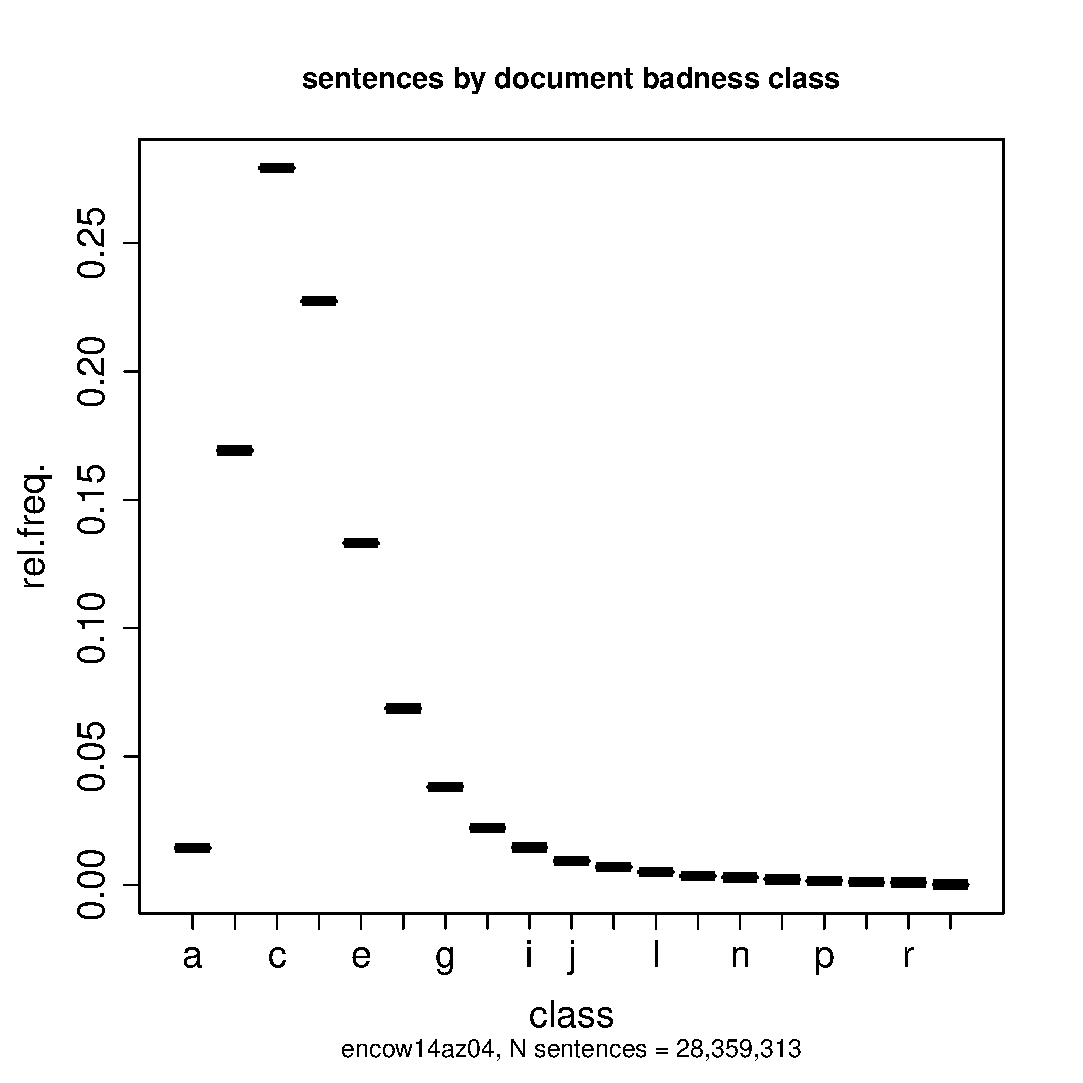
\includegraphics[height=0.9\textheight]{graphics/encow14az04_bdc}
\end{frame}



\begin{frame}
	\frametitle{Dokumentqualität: Subkorpora (ENCOW14AX)}
	\centering
	\begin{tabular}{lcl}
 		\textbf{Dokumentqualität} & \textbf{Klasse} & \textbf{Größe}\\
		\hline
	        gut           & $a-b$ & 100 M\\  
	 		mittel \& schlecht        & $f-s$ & 100 M\\
		\hline
	\end{tabular}
\end{frame}


%\begin{frame}
%  \frametitle{Boilerplate}
%  \centering
%  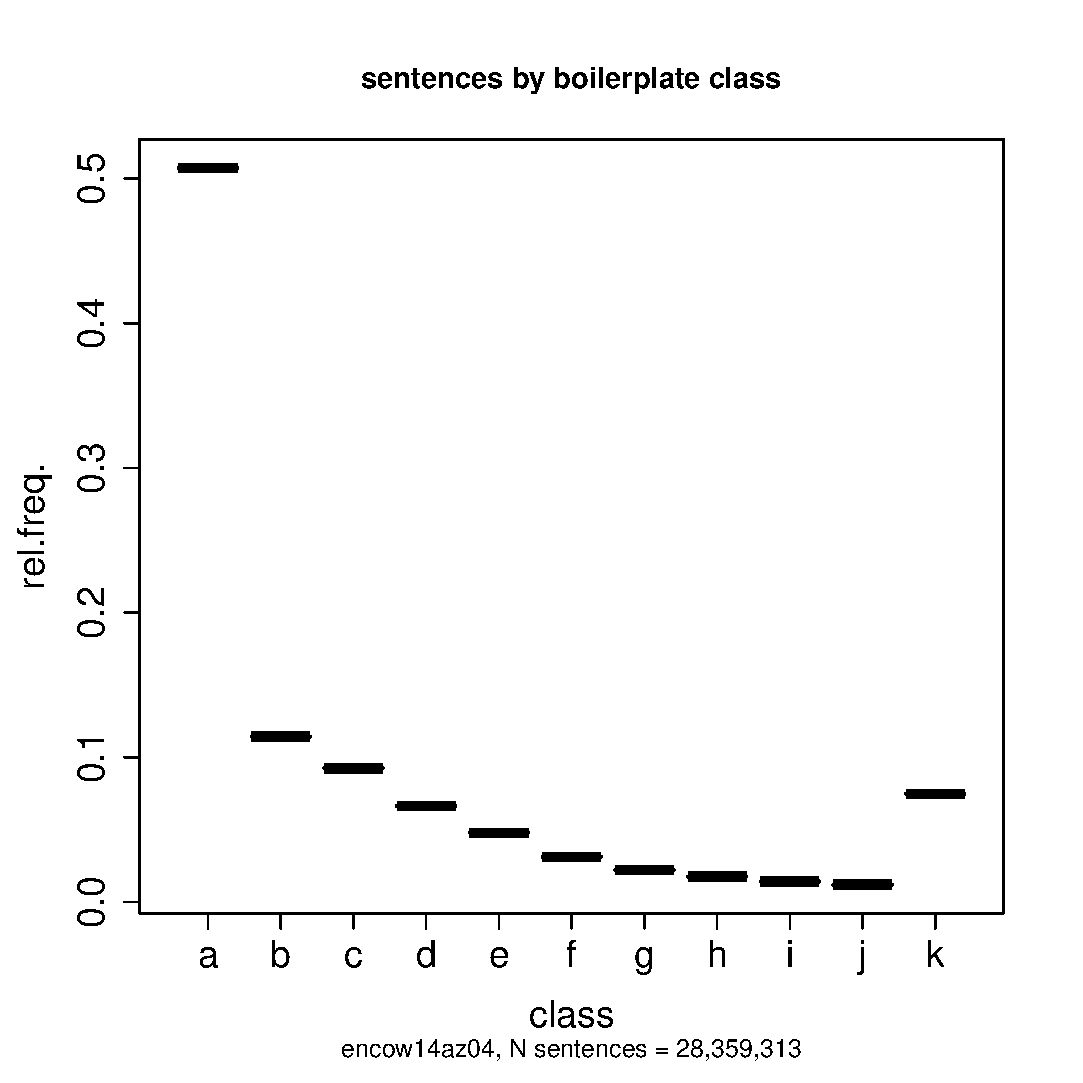
\includegraphics[height=0.9\textheight]{graphics/encow14az04_bpc}
%\end{frame}
%
%
%
%\begin{frame}
%	\frametitle{Boilerplate: Subkorpora (ENCOW14AX)}
%	\centering
%	\begin{tabular}{lcl}
%	 \textbf{Absatzqualität} & \textbf{Klasse} & \textbf{Größe}\\
%	\hline
%	             gut           & $a$ & 100 M\\  
%	 mittel \& schlecht          & $f-k$ & 100 M\\
%	\hline
%	\end{tabular}
%\end{frame}
%


%\begin{frame}
%	{Vorverarbeitung}
%	
%	ENCOW14AX  
%	
%	  \begin{itemize}
%	  \item einzelne Sätze
%	  \item Lemmatisierung (TreeTagger) 
%	  \item Entfernung von Satzzeichen
%	  \end{itemize}
%	
%	\pause
%	\vspace{1cm}
%	
%	BNC (100 M)
%	
%	\begin{itemize}
%	\item einzelne Sätze
%	\item bestehende Lemmatisierung
%	\item Entfernung von Satzzeichen
%	\end{itemize}
%\end{frame}
%
%
%\begin{frame}
%  \frametitle{Beispiel}
%  \begin{tabular}{ll}
%	   1 & \texttt{\small build in the 1st century the arena hold up to @card@ spectator}\\
%	   2 & \texttt{\small Can anyone explain how this be good for society as a whole}\\
%	   3 & \texttt{\small when I preach in the mosque I tell them to stay away}
%  \end{tabular}
%\end{frame}


\begin{frame}
  \frametitle{Ergebnisse: Dokumentqualität}
	\begin{center}
	 \scalebox{0.6}{\begin{tabular}{ll|ll}
	\hline
	  \multicolumn{2}{c}{\textbf{gut}}  &  \multicolumn{2}{c}{\textbf{mittel \& schlecht}}\\
	                T-80 & T-142 & T-80 & T-142 \\
	\hline                   
	                            .66&.65&.59&.60\\
	                            .68&.65&.62&.60\\
	                            .68&.68&.59&.61\\
	                           .61&.61&.57&.54\\
	                            .62&.64&.59&.56\\
	                            .64&.65&.62&.58\\
	                            .65&.65&.54&.56\\
	                            .64&.65&.60&.59\\
	                            .65&.63&.62&.62\\
	                            .69&.65&.60&.58\\
	\hline
	   \textbf{.65}&\textbf{.65}&\textbf{.60}&\textbf{.59}\\
	\hline
	\end{tabular}}
	\end{center}
	\pause
	\vspace{.2cm}
	
	   \begin{itemize}
	   \item Sätze aus guten Dokumenten ergeben ein besseres DSM.
	   \item Oder: Die automatisch annotierte Dokumentqualität korreliert
	     mit der Qualität des DSM.
	   \end{itemize}
\end{frame}


%\begin{frame}
%  \frametitle{Ergebnisse: boilerplate}
%	  
%	\begin{center}
%	\scalebox{0.6}{\begin{tabular}{ll|ll}
%	\hline
%	  \multicolumn{2}{c}{\textbf{gut}}  &  \multicolumn{2}{c}{\textbf{mittel \& schlecht}}\\
%	                T-80 & T-142 & T-80 & T-142 \\
%	\hline                   
%	
%	.66&.65&.57&.56\\
%	.65&.65&.60&.59\\
%	.65&.65&.57&.56\\
%	.64&.62&.57&.58\\
%	.64&.62&.54&.55\\
%	.64&.62&.55&.53\\
%	.60&.60&.59&.57\\
%	.65&.64&.59&.56\\
%	.66&.63&.59&.56\\
%	.62&.63&.52&.54\\
%	
%	\hline
%	\textbf{.64}&\textbf{.63}&\textbf{.57}&\textbf{.56}\\
%	\hline
%	\end{tabular}}
%	\end{center}
%	
%	\pause
%	\vspace{.2cm}
%	
%	   \begin{itemize}
%	   \item Sätze aus guten Absätzen ergeben ein besseres DSM.
%	   \item Oder: Die automatisch annotierte boilerplate-score korreliert
%	     mit der Qualität des DSM.
%	   \end{itemize}
%\end{frame}


\begin{frame}
	\frametitle{Vergleich: BNC}
	 
	\begin{center}
	\scalebox{0.8}{\begin{tabular}{ll}
	\hline
	  \multicolumn{2}{c}{\textbf{BNC}}\\
	                T-80 & T-142 \\
	\hline                
	.56&.56\\
	.58&.59\\
	.57&.59\\
	.58&.57\\
	.58&.60\\
	.59&.59\\
	.59&.59\\
	.58&.59\\
	.61&.61\\
	.59&.61\\
	\hline
	\textbf{.58}&\textbf{.59}\\
	\hline
	\end{tabular}}
	\end{center}
\end{frame}


%\begin{frame}
%  \frametitle{Vergleich: a-b/a Korpus}
%  \begin{itemize}
%  \item Ist der positive Effekt von guter Dokumentqualität und guter
%    Absatzqualität kumulierbar?
%  \item neues Subkorpus: Sätze nur aus guten Absätzen (Klasse $a$) in
%    guten Dokumenten (Klassen $a$ und $b$)
%  \end{itemize}
%	\begin{center}
%	\scalebox{0.6}{\begin{tabular}{ll}
%	\hline
%	  \multicolumn{2}{c}{\textbf{a-b/a}}\\
%	                T-80 & T-142 \\
%	\hline               
%	0.65&0.65\\
%	0.61&0.62\\
%	0.63&0.65\\
%	0.64&0.63\\
%	0.65&0.63\\
%	0.65&0.61\\
%	0.64&0.65\\
%	0.63&0.63\\
%	0.61&0.62\\
%	0.64&0.62\\
%	\hline
%	\textbf{.63} & \textbf{.63}\\
%	\hline
%	\end{tabular}}
%	\end{center}
%\end{frame}


\begin{frame}
	{Zusammenfassung}
  \begin{itemize}
  \item Ergebnis ist signifikant besser als der Zufall
%  \item Scheinbar keine Unterschiede zwischen Subkorpus/Nachverarbeitungs-Varianten
%  \item Unterschiede sind nicht signifikant
%  \end{itemize}
%%
%	\pause
%	\vspace{.25cm}
%	
%	\begin{itemize}
%	\item Beste Ergebnisse mit mittelgroßen Trainingskorpora\\%
%	  (ca.\  0.5 Mrd.\ Tokens), und ausschließlich guten Dokumenten
	\item Zukünftige Evaluationen mit DS:
	  \begin{itemize}
		  \item andere Tests
		  \item andere DS-Algorithmen
	  \end{itemize}
	
	\end{itemize}
\end{frame}

